\part{Binary notation}
\frame{\partpage}

\begin{frame}
	\centering
	\includegraphics[width=0.7\textwidth]{10-types-of-people}
	\par\vspace{2ex}\par
	{\tiny Image credit: \url{http://www.toothpastefordinner.com}}
\end{frame}



\begin{frame}{How we write numbers}
	\begin{itemize}
		\pause\item We write numbers in \textbf{base~10}
		\pause\item We have 10 \textbf{digits}: $0, 1, 2, \dots, 8, 9$
		\pause\item When we write $6397$, we mean:
			\begin{itemize}
				\pause\item Six thousand, three hundred and ninety seven
				\pause\item (Six thousands) and (three hundreds) and (nine tens) and (seven)
				\pause\item $(6 \times 1000) + (3 \times 100) + (9 \times 10) + (7)$
				\pause\item $\left(6 \times 10^3\right)
				+ \left(3 \times 10^2\right)
				+ \left(9 \times 10^1\right)
				+ \left(7 \times 10^0\right)$
				\pause\item
				    \begin{tabular}{cccc}
				        Thousands & Hundreds & Tens & Units \\
				        6 & 3 & 9 & 7
				    \end{tabular}
			\end{itemize}
	\end{itemize}
\end{frame}

\begin{frame}{Binary}
	\begin{itemize}
		\pause\item Binary notation works the same, but is \textbf{base~2} instead of \textbf{base~10}
		\pause\item We have 2 \textbf{digits}: $0, 1$
		\pause\item When we write $10001011$ in binary, we mean: \par\pause
			$\phantom{+} \left(1 \times 2^7\right) + 
			\left(0 \times 2^6\right) + 
			\left(0 \times 2^5\right) + 
			\left(0 \times 2^4\right)$ \par
			$+ \left(1 \times 2^3\right) + 
			\left(0 \times 2^2\right) + 
			\left(1 \times 2^1\right) + 
			\left(1 \times 2^0\right)$ \par\pause
			$= 2^7 + 2^3 + 2^1 + 2^0$ \par\pause
			$= 128 + 8 + 2 + 1 \text{ (base 10)}$ \par\pause
			$= 139 \text{ (base 10)}$
	\end{itemize}
\end{frame}

\begin{frame}{Converting to binary}
    \begin{center}
        \url{https://www.youtube.com/watch?v=OezK_zTyvAQ}
    \end{center}
\end{frame}

\begin{frame}{Bits, bytes and words}
	\begin{itemize}
		\pause\item A \textbf{bit} is a \uline{b}inary dig\uline{it}
			\begin{itemize}
				\pause\item Can store a 0 or 1 (i.e.\ a boolean value)
			\end{itemize}
		\pause\item A \textbf{byte} is 8 \textbf{bits}
			\begin{itemize}
				\pause\item Can store a number between 0 and 255 in binary
			\end{itemize}
		\pause\item A \textbf{word} is the number of bits that the CPU works with at once
			\begin{itemize}
				\pause\item 32-bit CPU: 32 bits = 1 word
				\pause\item 64-bit CPU: 64 bits = 1 word
			\end{itemize}
		\pause\item An $n$-bit word can store a number between 0 and $2^{n} - 1$
			\begin{itemize}
				\pause\item $2^{16}-1 = 65,535$
				\pause\item $2^{32}-1 = 4,294,967,295$
				\pause\item $2^{64}-1 = 18,446,744,073,709,551,615$
			\end{itemize}
	\end{itemize}
\end{frame}

\newcommand{\carry}[1]{\uncover<#1->{$_1$}}
\newcommand{\nocarry}[1]{\phantom{$_1$}}

\begin{frame}{Addition with carry}
	In base 10:
	\begin{center}
		\begin{tabular}{lllll}
			& 1 & 2 & 3 & 4 \\
			+ & 5\nocarry{4} & 6\carry{3} & 7\carry{2} & 8\nocarry{1} \\\hline
			& \uncover<5->{6} & \uncover<4->{9} & \uncover<3->{1} & \uncover<2->{2}
		\end{tabular}
	\end{center}
\end{frame}

\begin{frame}{Addition with carry}
	In base 2:
	\begin{center}
		\fbox{$1 + 1 = 10$ \qquad $1 + 1 + 1 = 11$}
		
		\vspace{2ex}
		
		\begin{tabular}{lllllllll}
			& 0 & 1 & 1 & 0 & 1 & 1 & 1 & 0 \\
			+ &
				0\carry{8} &
				0\carry{7} &
				1\nocarry{6} &
				0\carry{5} &
				0\carry{4} &
				1\carry{3} &
				1\nocarry{2} &
				1 \\\hline
			&
				\uncover<9->{1} &
				\uncover<8->{0} &
				\uncover<7->{0} &
				\uncover<6->{1} &
				\uncover<5->{0} &
				\uncover<4->{1} &
				\uncover<3->{0} &
				\uncover<2->{1}
		\end{tabular}
	\end{center}
\end{frame}

\begin{frame}{Modular arithmetic}
    \begin{columns}
        \begin{column}{0.4\textwidth}
            \begin{center}
                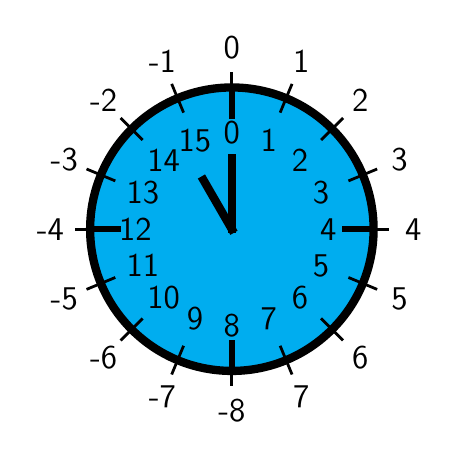
\begin{tikzpicture}[line cap=rect,line width=3pt,scale=0.9]
                    \filldraw [fill=cyan] (0,0) circle [radius=2cm];
                    \foreach \angle [count=\xi from 0] in {90,67.5,...,-247.5}
                    {
                        \draw[line width=1pt] (\angle:1.8cm) -- (\angle:2.2cm);
                        \node[font=\large] at (\angle:1.36cm) {\textsf{\xi}};
                    }
                    \foreach \angle [count=\xi from -8] in {270,247.5,...,-67.5}
                    {
                        \node[font=\large] at (\angle:2.56cm) {\textsf{\xi}};
                    }
                    \foreach \angle in {0,90,180,270}
                        \draw[line width=2pt] (\angle:1.6cm) -- (\angle:2cm);
                    \draw (0,0) -- (120:0.8cm);
                    \draw (0,0) -- (90:1cm);
                \end{tikzpicture}
            \end{center}
        \end{column}
        \begin{column}{0.55\textwidth}
            \begin{itemize}
                \pause\item Arithmetic \textbf{modulo} $N$
                \pause\item Numbers ``wrap around'' between $0$ and $N-1$
                \pause\item E.g.\ modulo $16$:
                    \begin{itemize}
                        \pause\item $14 + 7 = 5$
                        \pause\item $4 - 7 = 13$
                    \end{itemize}
            \end{itemize}
        \end{column}
    \end{columns}
\end{frame}

\begin{frame}{2's complement}
    \begin{itemize}
        \pause\item How can we represent negative numbers in binary?
        \pause\item Represent them modulo $2^n$ (for $n$ bits)
        \pause\item I.e.\ represent $-a$ as $2^n-a$
        \pause\item Instead of an $n$-bit number ranging from $0$ to $2^n-1$, it ranges from $-2^{n-1}$ to $+2^{n-1}-1$
        \pause\item E.g.\ 16-bit number ranges from $-32768$ to $+32767$
        \pause\item Note that the left-most bit can be interpreted as a \textbf{sign} bit:
            $1$ if negative, $0$ if positive or zero
    \end{itemize}
\end{frame}

\begin{frame}{Converting to 2's complement}
    \begin{itemize}
        \pause\item Convert the absolute value to binary
        \pause\item Invert all the bits (i.e.\ change $0 \leftrightarrow 1$)
        \pause\item Add 1
        \pause\item (This is equivalent to subtracting the number from $2^n$... why?)
        \pause\item This is also the process for converting back from 2's complement,
            i.e.\ doing it twice should give the original number
    \end{itemize}
\end{frame}

\begin{frame}{Why 2's complement?}
    \begin{itemize}
        \pause\item Allows all addition and subtraction to be carried out modulo $2^n$
            without caring whether numbers are positive or negative
        \pause\item In fact, subtraction can just be done as addition
        \pause\item I.e.\ $a-b$ is the same as $a+(-b)$, where $a$ and $-b$ are just $n$-bit numbers
    \end{itemize}
\end{frame}
